\svnkwsave{$RepoFile: siminos/baroclinic/OrtegaBlog.tex $}
\svnidlong {$HeadURL$}
{$LastChangedDate$}
{$LastChangedRevision$} {$LastChangedBy$}
\svnid{$Id$}

\chapter{Convectively coupled waves}
\label{chap:OrtegaBlog}

\section{Introduction}
\label{sect:CCWs}

\begin{description}

\item[2012-02-08 Predrag] Please write an introduction to
the ``Convectively coupled waves'' suitable to inclusion into
your thesis: what they are, and why should one care. Add relevant references
to this repository's siminos/bibtex/siminos.bib (no separate bibliographies,
it makes updating them a pain).

\end{description}

\section{Sebastian's blog}
\label{sect:OrtegaDaily}

This is Sebastian Ortega Arango's blog for PHYS 7224,  spring 2012
\emph{Nonlinear dynamics: Chaos, and what to do about it?} course project

\begin{description}

\item[2012-02-07 Predrag] Added Sebastian Ortega Arango
<sortega@gatech.edu> project to this blog; enabled svn access, updates
(sortega  baroclinic). First task: please study \refchap{chap:baroclinic},
and improve it in any way you see fit, edit, add better references etc.

\item[2012-02-07 Sebastian]
I think I would be able to relate the project with my line of research. I
am interested in \textbf{Convectively Coupled Waves}. I read that people at NYU
has worked the mathematics in this types of phenomena, and it appears
that interesting nonlinearities arise from it. Baroclinic instability
seems to bee an important driver.

\item[2012-02-08 Predrag] I would like the project to focus on a
geophysically important model that exhibits $\SOn{2}$ invariance,
hence propose to investigate the baroclinic instability first, then apply
that to your thesis research on Convectively Coupled Waves. Advantage of
starting with the baroclinic instability is that you can hit the ground running,
as Annalisa has simulation code ready to use.

\item[2011-10-15 Annalisa] Define and explain the Rossby radius for the
atmosphere in \refsect{sect:CCWs}. Mark here [~~] when done.

\item[2012-03-27 Sebastian] I am going to follow your advice and star
working with baroclinic stability first. I have written a draft of the
introduction, the idea is that it outlines the work to be done, and is
subject to changes. I think it is a good outline to introduce baroclinic
instability, and to introduce the model used in the simulations. However,
it still not clear to me how to include the nonlinear analysis. I will
continue reading about the \KSe\ and the \pCf\ for this. I will try to
write \refsect{s:intro} today.

\item[2012-03-27 Predrag] I'm glad you are getting started - go for it.

\item[2012-03-27 Sebastian]
Also, I find a thesis that might be interesting to read Veen's thesis,
\HREF{http://igitur-archive.library.uu.nl/dissertations/2002-0801-151812/c2.pdf}
{Chapter 2}.

\item[2012-03-27 Predrag] I have not read Lennart's thesis, but he does good work. Blog
here what you find of interest as you read it.

\item[2012-04-04 Sebastian]
Finished first and second section. I am uploading to show what I have
done so far, but it is just a quick draft as far as redaction goes. I
still have to read it again and correct it. Some times I write in this
way, first I get all the ideas in paper and then iterate until I have a
coherent document. Probably not the best way out there.

In short, the point that I am trying to get trough, is that there is a
base flow given by geostrophy and the hydrostatic relation which might be
stable depending on the slope of the isopycnals. Then I introduce the
model Professor Annalisa used for her simulations (I believe is the one
described by Philips in 1951).

I think it is important for me to get focus on the nonlinear aspects of
the problem. So I will try to finish all the way to
\refsect{s:stability} by this week (but not sure if I will have the time).

I was also wondering what should I do for the nonlinear section. But I
guess I should first order my ideas and learn how to think of baroclinic
instability in terms of dynamical systems. So far I think of it from the
point of view of bifurcations (please correct me if wrong), where I have
a equilibrium point in the dynamical system which becomes unstable (or
disappears??) after some parameter increases (this is what I believe the
linear theory does). But I am not sure what happens once the flow is
unstable, my guess is that there would be some kind of strange attractor
out there in the n-dimensional space. But I guess visualization of this
would be quite hard, unless a low order spectral representation is used.
It would be very interesting to hear your vision of the instability; so
please let me know if there is a paper I can read for this, or what you
think is happening.

Also, let me know of any changes that you think might be convenient.

\item[2012-04-05 Sebastian]
A quote from Rick Salmon book (might be good for Chaos book). After
proving Ertel's Theorem: "Of course, we can prove all these results
directly from (1.1)
% \footnote{Momentum equation, continuity equation,
% thermodynamic equation and equation of state}
by pedestrian mathematical
manipulations, but that only makes it harder to appreciate their physical
significance" {\bf [2012-04-05] Predrag} added to the ChaosBook trove of
reserve quotes, thanks!

\item[2012-04-05 Sebastian]
Done with \refsect{s:stability} \emph{Stability theory} text. However,
some calculations are needed for the specific case (those for $\omega$
and $U_c$). But they might be in the literature somewhere; however there
should be easy to do (or reduce easily from the ones given by Hasha\rf{Hasha05}
and/or Vallis\rf{Vallis06}).

\item[2012-04-23 Sebastian]
I have been trying to figure out how to find the fixed points and
periodic orbits for my project. However, I am not really sure how to
implement Viswanath GMRES algorithm to Annalisa's code (maybe a simpler
one is ok, as Viswanath also look for relative periodic orbits). I think
I have to write a searching algorithm based on the method, so I have been
spending time trying to understand the solution method, although I have
not fully understood it yet. I also found Halcrow theses in the web, this
might help me figure out how to do it.

I think I will start writing down everything I have read, and what I
think it might be found for the model. And then try to do code the
searching algorithm. Let me know if you have any pointers for this, or if
I should do something differently.

\item[2012-04-23 Predrag]
I think implementing Viswanath GMRES algorithm to Annalisa's code is a
semester project. It might be easier to implement her code as a module in
channelflow.org, but that too is months of work. It is certainly worth
doing, but you cannot do it in a week. I am happy if in your project
right now you run her code, see some interesting structures, and maybe
manage to find a close recurrence in the data.

Read the end of siminos/blog/blog.tex, chapter {\em Fluids} about this.

\item[2012-04-23 Sebastian]
By the way, is there class tomorrow?

\item[2012-04-23 Predrag]
Yes, this is the last week. If people want to, they can self organize to present their
projects the coming week, but I'm not supposed to meddle, as it is exam week.

\item[2012-04-23 Sebastian]
I guess I got a little exited about the papers I read; very interesting. I will try then to limit the search to recurrent motions. But will write about what can be done in the future. I have ran Annalisa's code already, so I will try to search this by looking at dissipation and energy plots as done in Viswanath to find an initial guess for periodic orbits. But my guess is that it would be very qualitative.

I was wondering what you think the implications of periodic orbit theory are for climate and weather. I have the feeling that it must be very important. But would like to hear what you think about it. I want to study predictability for my Phd work, focusing on the tropics intraseasonal variations (MJO and such); exploring this kind of approaches seem as something important to me. Let me know when you have time to discus this and I will go by your office.

\item[2012-04-24 Sebastian]
Forgot to upload the blog yesterday. I am uploading it along with some advances in the nonlinear section (\refsect{s:nonlinear} not yet complete). Just the ideas of some important papers I have found; and what I intend in doing for Chaos project.
Currently I am running Annalisa's code for a longer period, 5 times more than before. And playing with the visualization of energies and dissipation to see if I can find close recurrences. I was also thinking in changing the parameters of the simulation. But I think I will try to find them first in the simulation as it is, and then change them if necessary.
Any suggestions or recommendations are welcome.

\item[2012-04-25 Predrag]
Here is my concrete proposal for what you can do now, for the course
project. What you have written is good. What would really help us
(Annalisa, me, you) is if you read the Chaos Gang paper (click
\HREF{http://www.cns.gatech.edu/~predrag/papers/preprints.html\#atlas12}{here}),
and implement the sliced version of Annalisa's simulations. You do not
need any invariant solutions to do this, use as a template a typical
turbulent state in the simulation.

The key physical step is choice of norm, read commentary after Eq. (1).
Slicing means that given the norm and the template, you replace ODE
integrator velocity fields by the ones in slice, Eq. (8): these videos
should be much calmer than the original simulation, as drifts have been
quotiented out. That is already enough to complete the term project.


Next keep track of phase velocity Eq (9). If that diverges it means you
are falling of the edge of your template's chart: you should use a
multiple chart atlas. If you get a few charts, ridges, and reduced flow that
encounters no singularities, we already have a publication.

Finding invariant solutions is essential, and cannot be done without
symmetry reduction, but it not necessary to illustrate symmetry
reduction.

\item[2012-04-25 Sebastian]
Will try to do so. But the representation as in \refeq{DS} is still not
clear to me from the code. The vorticity and the stream functions both
change in time and one depends on the other ($\xi=\nabla^2\phi$).
However, the equations are solved for the vorticity with a
Adams-Bashforth integration. So maybe I can just forget about the stream
functions and think of the system as
$d\widehat{\xi}/dt=F(\widehat{\xi},\nabla)$, but I am not sure. For this
I should derive the equations used in the spectral method, so I have to
study more about it first; in the code FFT is used in several steps, so
the exact form of the spectral equations is not completely clear for me.
Thus, I am not sure how to compute the generator \Lg\ either.
Let me know if you have any advice for this.

\item[2012-04-25 Predrag] Whatever Adams-Bashforth integration are your
\statesp\ coordinates. The FFT must be used in the stream-wise direction -
when you are in the Fourier representation, use this to implement a rotation
on each mode separately.

                                                    \toCB
For the one-parameter rotation group \SOn{2}
acting on a smooth periodic function $u(\gSpace + 2\pi) = u(\gSpace)$
defined on domain $x
\in [0,2\pi)$ we can be explicit. The
\statesp\ matrix representation of the \SOn{2}\ rotation $\LieEl(\phi)
u(\gSpace) = u(\gSpace+\phi)$ by angle $\phi$ is block-diagonal, acting
on the $m$th Fourier coefficient pair $(a_m,b_m)$ in the Fourier series,
\beq
u(\gSpace) = a_0 + \sum_{m=1}^\infty \left(
a_m \cos m \gSpace + b_m \sin m \gSpace
                               \right)
\,,
\ee{FourierExp}
by multiplication by
\beq
\LieEl^{(m)}(\phi) \,=\,  \left(\barr{cc}
 ~\cos m \phi  & \sin m \phi \\
 -\sin m \phi  & \cos m \phi
    \earr\right)
                \,,\qquad
\Lg^{(m)} \,=\,   \left(\barr{cc}
    0  &  m  \\
   -m  &  0
    \earr\right)
\,.
\ee{SO2irrepAlg-m}
%\ee{SO2irrepAlg-Lg}
In complex representation
the shifts along the streamwise periodic direction
$z$ is given by
\beq
   \vec{u}' = \LieEl(\phi,\shift) \vec{u} \, : \qquad
   \vec{u}_{nkm}' = \vec{u}_{nkm} \,
   \mathrm{e}^{-\mathrm{i}(m_0 m\phi+\alpha k \shift)} ,
\eeq
The $\SOn{2}$ group tangent to \statesp\ point $\ssp$ within the $m$th
invariant subspace is
\beq
 \groupTan^{(m)}(\ssp)
\,=\, m \,\left(\barr{c}
   ~b_m  \\
   -a_m
    \earr\right)
\,.
\ee{u:x:tang}

\item[2012-04-25 Predrag] You might want to form a Slicers (Slashers? a
word we have not misused yet) Anonymous Support Group with Luis - he is
supposed to doe exactly the same PDE slicing as you, except his symmetry
is $E(2)$ Euclidean group. In his case I suggested that he does not touch
the code, but post-process by turning the full space trajectory into the
\slice\ by finite angles.

\item[2012-04-29 Sebastian]
I have been having a bit of trouble figuring out how to calculate the
moving frame for each point. However, I think I am close to make it.
Here is how I have been trying to do it: I have been using the
postprocessing approach converting the vorticity output from the model
back to spectral space with a fast sine transform for Y and a fast
fourier transform for X (I think this is how it's done in Annalisa's
code). The results of the transform are shown in \reffig{f:fouriervort}.

    \begin{figure}[t]
    \begin{center}
    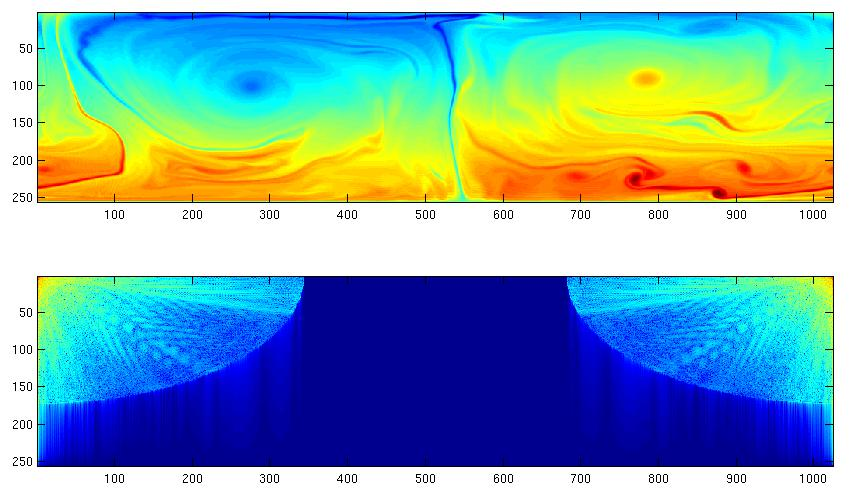
\includegraphics[width=0.9\textwidth, clip=true]{fouriervort}
    \end{center}
    \caption{(top) Vorticity field. (bottom) Spectral representation
    ($ln(1+abs(\xi))$). Note that some frequencies are just the complex
    conjugate of others.}
    \label{f:fouriervort}
    \end{figure}

This means that the vorticity can be expressed as:
    \PC{$a(l)_{k}$ stands for $a(y,t)_{k}$, \ie, coefficients carry spanwise
        and time dependence? Or what is this $l$?}
    \beq
    \xi(x,y)=\sum a(l)_{k} e^{-2 i \pi k x/M}
    \ee{120429_1}
So as stated in \refref{ACHKW11}, $\LieEl(\gSpace)=diag(e^{-2 \pi i k \gSpace /M})$
and $\Lg=diag(-2 \pi i k/M)$.

Now, the slice condition is given by $\LieEl( a_{kl}^T \gSpace(t))^T \Lg \slicep_{kl}$,
so I express the matrix as a vector:
    \beq
    a_{kl}=
    \begin{pmatrix}
    a_{11} & a_{12}& \cdots & a_{1N}&\cdots&a_{MN}\\
    \end{pmatrix}^T
    \ee{120429_2}
and carry out the slice condition, which looks something as:
    \bea
    \begin{pmatrix}
    a_{11} \\ a_{12}\\ \cdots \\ a_{1N}\\\cdots\\a_{MN}\\
    \end{pmatrix}^T
    \begin{pmatrix}
    e^{-2 \pi i \gSpace /M} & 0& \cdots & 0\\
    0 &  e^{-4 \pi i \gSpace /M}& \cdots & 0\\
    \vdots & \ddots& \ddots & \vdots\\
    0 & 0& \cdots & e^{-2 N \pi i \gSpace /M}
    \end{pmatrix}\\
    \continue
    \cdot
    \begin{pmatrix}
    -2 \pi i /M & 0& \cdots & 0\\
    0 &  -4 \pi i \gSpace /M& \cdots & 0\\
    \vdots & \ddots& \ddots & \vdots\\
    0 & 0& \cdots & -2 N \pi i  /M
    \end{pmatrix}
    \begin{pmatrix}
    \slicep_{11} \\ \slicep_{12}\\ \cdots \\ \slicep_{1N}\\\cdots\\\slicep_{MN}\\
    \end{pmatrix}^T = 0
    \label{120429_3}
    \eea
which after carrying it out gives me something as (but I have to check the algebra):
    \beq
    \LieEl(\gSpace(t))^T a_{kl}^T T \slicep_{kl}
     =\sum_{n=1} \left[n e^{-i n \gSpace}\left(\sum_{m=1}a_{mn}\slicep_{mn}\right)\right]=0
    \ee{120429_4}
I guess the next step would be to apply a Newton-Raphson to
\refeq{120429_4}. However, I am not sure how this would work, as the
equation have quite a large amount of terms, and has also an imaginary
component. Let me know if you have any advice for this.

Note: I will check the algebra tomorrow again; most likely I made an
embarrassing amount of mistakes while writing this. It is to late now.

\item[2012-04-29 Predrag]
You rotate only the fast Fourier transform for X, there is no
translational symmetry in the Y direction.

A vector is a vector, both in space and in Fourier space, so I do not see
why $a_{mn}$ became a matrix. Hope this helps (real form - complex is even
simpler):

Consider the general action of an
$\SOn{2}$ symmetry on arbitrary Fourier coefficients of a spatially
periodic function. Substituting this into the slice
condition
and using $g^{(m)}(\gSpace)=\cos(m\gSpace)\id^{(m)} +\sin(m\gSpace)
\frac{1}{m}\Lg^{(m)}$, we find that
\bea
\braket{e^{-\gSpace \Lg}\ssp}{\groupTan(\slicep)}
=\braket{\ssp}{\sum\limits_m \left(\cos(m\gSpace) \id^{(m)}
     +\sin(m\gSpace) \frac{1}{m}\Lg^{(m)}\right) \sliceTan{}}
\continue
=\sum\limits_m
   \left(
    \braket{\ssp}{\Lg^{(m)} \slicep} \cos(m\gSpace)
  - m\braket{\ssp}{\id^{(m)} \slicep} \sin(m\gSpace)
   \right)
   =0
\,.
\label{eq:so2sing}
\eea
This is a polynomial equation, with coefficients determined by
$\braket{\ssp}{\Lg^{(m)} \slicep}$ and $\braket{\ssp}{\id^{(m)}\slicep}$,
as we can see by rewriting $\cos(m\gSpace)$, $\sin(m\gSpace)$ as
polynomials of degree $m$ in $\sin(\gSpace)$ and $\cos(\gSpace)$. Each
phase $\gSpace$ that rotates $\ssp$ into any of the group-orbit
traversals of the slice hyperplane corresponds to a real root of this
polynomial.

It is fast - just a dot product, and as $\gSpace$ dependence is only in
the group element, the $d/d\gSpace$ derivative you need for Newton.
Complex Newton formula is the same as for real functions, thanks to
analyticity (analyticity assures that complex derivatives make sense).

\item[2012-04-30 Sebastian]
I do not understand why the transpose gets replaced by a complex
conjugate. I see in matlab what you mean by the transpose of the matrix.
But why does the complex conjugate gets involved in the transpose.

\item[2012-04-30 Predrag] If you are going to work in complex
representation, the norm of a complex vector $\ssp \in \complex^d$ is
$\norm{\ssp}^2 = \ssp^* \cdot \ssp$, and $(\LieEl\ssp)^*
=\ssp^*\LieEl^\dagger$, where $\LieEl^\dagger$ is the hermitian conjugate
= transpose + complex conjugate.

\item[2012-04-30 Predrag] Before getting into the Newton for this - make
sure that your $\LieEl(\gSpace)$ applied to a baroclinic state $\ssp$
does shift it by $\gSpace$, \ie,  $\LieEl(\gSpace)\ssp$ is the same $2D$
picture, but shifted by $\gSpace$.

\item[2012-04-30 Sebastian]
I have made a Matlab code that shifts the image by a $\gSpace$. Using
$\LieEl(\gSpace)=diag(e^{-2 \pi i k \gSpace /M})$. Looks as expected when converted
back to physical space.

\item[2012-04-30 Sebastian]
I reshape a matrix into a vector as Matlab's FFT works by columns. What I
have is a matrix that represents a vorticity field \SOA{which actually is
given as a vector from Annalisa's code, but I reshape it into a matrix
before doing anything in matlab} so what I do is to make a Fast Sine
Transform (FST) in Y and a FFT in X. This is something similar to
performing a 2D FFT. But to move all the fourier coefficients in X, I
reshape everything again as a vector. And then carry out the slicing
condition (all this in paper, in Matlab I have go up to the FFT transform
representation). So I think this would be equivalent only to a shift in
X.

Vector turns out to be huge, $262144$ dimensions for complex numbers; so
really is like $524288$ dimension. But a bit less than half of them are
just complex conjugates.

The term $a(l)_{k}$ means actually $a(l, t)_{k}$. I use it just to
emphasize that the transform in $x$, which is related with $k$, is
performed after a FST is made on the data for the $y$ direction. The
subindex $l$ is related to $y$. So $a(l)_{k}$, or perhaps better to write
$a_{lk}$, is a matrix (as shown in \reffig{f:fouriervort}), that I have
to reshape to rotate into the slice.  But I am not really sure why you
think it should be a vector.

\item[2012-04-30 Predrag]
Not sure why things got so huge? No point using Matlab for this - it is
fast and simple writing a dot product in C++ or Fortran. This is
Annalisa's department.

\item[2012-04-30 Sebastian]
I think the general procedure of what I did yesterday is OK. I have been
making the calculations this morning again. I believe is similar to what
you did in \refeq{eq:so2sing}, just that in complex space. By the way,
how do you get $e^{-\gSpace \Lg}$ to multiply $t'$ directly? Is it
because there should be a transpose in $e^{-\gSpace \Lg} x$?

%\item[2012-04-30 Sebastian] Advise greatly appreciated.
%\item[2012-04-30 Predrag] `advise' $\to$ `advice'.

\item[2012-04-30 Predrag] To view just the project (without this blog)
toggle the \texttt{boyscoutfalse} switch, towards the top of
\texttt{siminos/baroclinic/BrCv12.tex} file.

\item[2012-04-30 Sebastian]
How do you show that $\slicep^\dagger \Lg \slicep =0$?

\item[2012-04-30 Sebastian, Predrag]                                            \toCB
Unitary transformations preserve the magnitude of a complex vector
$\norm{\ssp} = \norm{\LieEl(\gSpace)\ssp}$, so $\LieEl^\dagger\LieEl=1$.
Expanding the norm to leading order in $\gSpace$
$\braket{(1+\gSpace\Lg)}{(1+\gSpace\Lg)}$ shows that the generators
are antihermitian, $\Lg^\dagger = - \Lg$, and from that it follows by complex conjugation
of the dot product $\ssp^\dagger \Lg \ssp$ that
$\ssp^\dagger \Lg \ssp =0$ for any vector $\ssp \in \reals^d$.

To evaluate the slice condition for unitary groups,
\beq
\frac{\partial}{\partial \gSpace} \norm{\ssp-\LieEl\slicep}^2 =0
\,,
\ee{120429_5}
start by expanding
\[
    (\ssp-\LieEl\slicep)^\dagger (\ssp-\LieEl\slicep)
= \norm{\ssp}^2
  - \slicep^\dagger\LieEl^\dagger\ssp - \ssp^\dagger\LieEl\slicep
  + \norm{\slicep}^2
\]
 so
\bea
\frac{\partial}{\partial \gSpace}
    (\ssp-\LieEl\slicep)^\dagger (\ssp-\LieEl\slicep)
&=& -\frac{\partial}{\partial \gSpace}
(\slicep^\dagger\LieEl^\dagger\ssp + \ssp^\dagger\LieEl\slicep)
 = -2\,\Re \left(\ssp^\dagger \frac{\partial \LieEl}{\partial \gSpace} \slicep\right)
\continue
&=& - 2\,\Re \left(\ssp^\dagger \LieEl \Lg \slicep\right)
\,.
\label{120429_6}
\eea
Substitute $\ssp=\LieEl\sspRed$.
    \PC{This is OK for abelain groups, as along the way I assumed $\LieEl
    \Lg = \Lg\LieEl $, but have to redo it more carefully for nonabelian
    groups.}
This yields the \emph{slice condition} for unitary groups:
\beq
    \Re(\sspRed^\dagger \Lg \slicep)=0
\ee{120430_11}
%\beq
%\frac{\partial}{\partial \gSpace}
%\left(\ssp^\dagger a - a^\dagger g\slicep -(g\slicep )^\dagger a+(g\slicep)^\dagger g\slicep \right)
%\,,
%\ee{120429_7}
%carrying out the derivative, nothing that $\partial g/\partial \gSpace =
%\Lg g$ and grouping terms I arrive to:
%\beq
%(\ssp-g\slicep)^\dagger \Lg \LieEl\slicep +(\Lg \LieEl\slicep)^\dagger (\ssp-g\slicep )=0
%\,.
%\ee{120429_8}
%As both terms are a complex numbers and one is the complex conjugate of
%the other, this means that the imaginary term vanish and the condition
%can be written:
%\beq
%2 \Re[(\ssp-g\slicep)^\dagger \Lg \LieEl\slicep ]=0
%\,,
%\ee{120429_9}
%and $a=g\widehat{\ssp}$, so that
%\beq
%2 \Re[(\widehat{\ssp}-\slicep)^\dagger g^\dagger \Lg \LieEl\slicep]=0
%\ee{120429_10}
%but
%$g^\dagger=diag[\overline{e^{-im\gSpace}}]=diag[e^{\overline{-im\gSpace}}]
%=diag[e^{im\gSpace}]$ so that $g^\dagger \Lg g=\Lg$ an the condition becomes:
%\beq
%2 \Re[(\widehat{\ssp}-\slicep)^\dagger \Lg \slicep ]=0
%\ee{120429_11}
One use this condition for Newton-Raphson determination of \sspRed.

\item[2012-04-30 Sebastian]
I tried to run the model changing the resolution, but results
do not look \PCedit{good}. Not much happened, energy did not traveled up scale.
Small scales are important. I think the simulation starts looking good
from $512 \times 128$ so I might change to that one. But there is always the
chance that I did not change some parameter in the simulation needed when
changing scales. I would have to check with Annalisa.

\item[2012-04-30 Sebastian]
Not sure $\ssp^\dagger \Lg \ssp$ vanishes, although it is antihermitian
it is a diagonal matrix. I think the correct answer is:
\beq
\ssp^\dagger \Lg \ssp = - \sum_{l=1} \sum_{k=1} i k \| \ssp_{l,k}\|^2
\ee{anti-antihermiticity}
Let me know if I am missing something.

\item[2012-05-01 Predrag]
Maybe elementary, student Ortega. Take $[1\!\times\!1]$ antihermitian matrix $\Lg = \ii$.
It's diagonal, right. And  $\Lg^\dagger = - \ii$. If we did this as $\SOn{2}$ there would be
no confusion, but with $\Un{1}$ one tends to get confused. BTW, there is no sum on $l$ in
\refeq{anti-antihermiticity} - it vanishes for every value of $l$ separately.

$\ssp^\dagger \Lg \ssp= (x-\ii y)\ii (x+\ii y) = $

\item[2012-04-30 Sebastian]
Ok. So a'+Ta' vanishes? I do not see it. I can go by your office and tell
you how I derive it, maybe you can tell me where I went wrong. The sum in
l is an artifact of how I derived things.

\item[2012-05-1 Sebastian]
Finish writing a very quick draft of the non linear section.

\item[2012-05-1 Sebastian]
Did some tweaking for the final project. Now it is in final form. I did
not have time to check all equations, but I guess they are ok. I will go
after Thursday trough the derivation of \refeq{min4} and run the
algorithm to see what happens.

I think it turn out ok. I like the final result. Let me know what you
think. As usual comments are greatly appreciated.

\item[2012-05-4 Sebastian]
I have been trying to implement the slicing condition of the term
project. Newton method converges and it is quite fast, even for the
1024x256 runs. However, it always converges very near the initial guess,
so that something is wrong. I was also thinking of how is one to
implement the {\chartBord} condition given that we are dealing with complex
numbers.

\item[2012-05-04 Predrag] If you are going small steps in time, this
sounds right - the in-slice trajectory will be close to the full space
trajectory. You just have to be sure that all points on it satisfy the
slice condition.

\item[2012-05-04 Sebastian] Let me know if you have any advise for any of
these points.

%\item[2012-04-30 Predrag] `advise' $\to$ `advice'.

\item[2012-05-04 Sebastian]
I spotted some things I can correct in my final work (minor changes), let
me know if changes are still allowed.

\item[2012-04-30 Predrag]
Keep editing and improving it - I can always post improved version on
\HREF{http://ChaosBook.org/projects}{ChaosBook.org/projects}. As far as I
am concerned, this project is not over until either the fat lady sings,
or you slice the baroclinic instability.

\item[2012-05-05 Sebastian]
% Sorry I keep misspelling `advice'. I will get it right next time.
Not sure if $\gSpace$ is correct. I am using all the time steps of the
simulation. If I start at $\gSpace=0$ then the algorithm converges to
something near $0.1$  for the next step; but from looking at the
simulations, if the drifting where to be removed, I think $\gSpace$
should be around $50$ as the transformations are made using
$\LieEl=\textrm{diag}\{e^{-2 i \pi k \gSpace/N}\}$ where $N=1024$. Any
number less than unity for $\gSpace$ makes no sense.
\item[2012-05-05 Predrag]
To isolate the problem, maybe sidestep the integrator, replace it by any
instantaneous state that you shift using the translation operator
(instead of integrating the PDEs). That is a mock-up of a \reqv, and your
Newton should make it stationary in the \slice.
\item[2012-05-05 Sebastian]
The sidestep approach should be a good test. I will also try that.
% Let me know what you think. As always any advice is welcome.

\item[2012-05-05 Sebastian]
I use \refeq{min4} for the slice condition in Newton Method. But I am not
sure how to implement the {\chartBord} condition for complex vectors. I
will work something out. In the moment I am calculating the real part of
the condition.

\item[2012-05-05 Predrag] There is only one shift $\gSpace$ to compute -
it fixes both the real and imaginary parts of the $\Un{1}$
transformation.
% If by `transversality condition' you mean the
% {\chartBord} condition \refeq{sliceSingl0},
The dot product is the usual
$L2$ one, in the streamwise direction
\beq
  \Norm{\ssp-\ssp'}^2  = \braket{\ssp-\ssp'}{\ssp-\ssp'} =
\Lint{\pSpace} ({u}-{u}')^\dagger \cdot ({u}-{u}')
\,.
\label{CmplxNorm}
\eeq

\item[2012-05-05 Sebastian]
I have been thinking about the reason my post-processing slicing does not
work. I went over the code and derivation today, but couldn't find what
is wrong with it.
So I think it is not an implementation issue but something else.  Maybe
in this case (after the FFT is used), it might not be correct to regard
the moving frame as continuous variable; as the rotation of the FFT
only makes sense (and only works) when the moving frame is an integer
($\gSpace$ in \refeq{min4}). This way, we might need a discrete version
of the Newton-Raphson algorithm.

I will search for an algorithm for this; although it should be easy to
create one from scratch; we just have to evaluate $\gSpace$ in
\refeq{min4} from $1$ to $1024$, and see where the values goes from
positive to negative. If we select a good initial value for \refeq{min4},
and if we are lucky enough, then it should work. We won't be able to find
a value that makes \refeq{min4} zero, but this is a resolution issue.
Note also that we do not always need to evaluate $\gSpace$ in
\refeq{min4} form $1$ to $1024$. With a good initial guess fewer points
should be necessary.

\item[2012-05-05 Predrag]                                   \toCB
Mhm - I have been wondering about this since 1993, when Eckhardt and
I\rf{CvitaEckardt} worked out how to
\HREF{http://ChaosBook.org/paper.shtml\#discrete} {quotient discrete
symmetries}. There you learn that if you can cut a `pizza' into $n$
equivalent slices, you should work in a single sliver, or fundamental
domain. I tried to quotient $\SOn{2}$ as a limit $ n \to \infty$ of
discrete cyclic group symmetry $\Zn{n}$ (in your case $n=1024$), and in
retrospect I believe it was a wrong path that kept me from doing the
right thing (slicing) for many years. The problem is that in the discrete
quotienting you make the \reducedsp\ smaller (by replacing the full
\statesp\ by a sliver) but the dimensionality of the space remains the
same. In reduction of continuous symmetries you decrease the dimension of
\statesp\ by one, for each continuous symmetry parameter. I do not see how
one would get to this $\lim_{n \to \infty} \Zn{n} = \SOn{2}$ limit by
the fundamental domain approach.
    \PC{to Predrag - copy this to pipes/blog}

I think what you should do is keep $\gSpace$ continuous, and interpolate,
meaning that in the Fourier rep you shift by the continuous phase, and
then FFT back to space; result will not be $j/1024$ shift but something
in between.

\item[2012-05-05 Predrag]                                   \toCB
We have the same problem in slicing experimental data - it is digitized,
and the slice condition will not respect the discrete pixel size, so
sliced video has to be re-digitized. As this can be done as
post-processing, I see no danger of introducing numerical errors into the
data set.


\item[2012-05-07 Sebastian]
I implemented a discrete Newton-Raphson method and it seems to work. I
think I have sliced baroclinic instability. Of course, I have to think
more about the {\chartBord} condition. I will upload the code at night
(I don't have my laptop in the office).

\item[2012-05-07 Predrag to Ashley] Do you understand why one would have a
\emph{discrete} Newton-Raphson? Do not even know what it means... In your pipe
slicing $\gSpace$ is continuous, right?


\item[2012-05-07 Sebastian] Here is the first animation of sliced baroclinic
instability:
    \PC{the animation is not in the repository to save space - if you
    want to have a look, I can place it in the DropBox.com}

\begin{quote}
\HREF{../movies/BaroclinicSlice.avi}{../movies/BaroclinicSlice.avi}.
\end{quote}

As expected, the slice seems to be useful only for a limited time. But
ignore the {\chartBord} condition in the moment. It might be correct,
but I have to check.

\item[2012-05-07 Predrag to Sebastian] Slicing does seem to stop the flow
from drifting, but otherwise not much simplification - it will be
hopefully more striking once you start plotting trajectories in the \statesp.

% Do not know what is the `transversality condition'. Do you mean
The
{\chartBord} condition \refeq{sliceSingl0} is
\[ %beq
\braket{\groupTan(\sspRSing)}{\sliceTan{}} \,=\, 0
\,.
% \label{sliceSingl0}
\] %\eeq
I'm bothered by $10^{-5}$ magnitude of whatever you are plotting. How about
plotting just the $\cos$ of the angle between the two tangent vectors,
\beq
\cos \theta = \frac{\Re
            \braket{\groupTan(\sspRSing(\zeit))}{\sliceTan{}}
                    }{
            \Norm{\groupTan(\sspRSing(\zeit))}\,\,{\Norm{\sliceTan{}}}
                    }
\,,
\label{chartBordAng}
\eeq
using \refeq{min5} and \refeq{min6}? Whenever this goes through zero,
$\sspRed(\zeit)=\sspRSing(\zeit)$, you have fallen off the {\chartBord}.
It should be doing it smoothly, as the \template\ is arbitrary, so there
is nothing special for the full \statesp\ trajectory happening at that
instant. Plot $\Norm{\groupTan(\sspRed(\zeit))}$ as well; it should also
vary smoothly, and \emph{not} get very small: if it does, alert me - it indicates
that you the trajectory is passing very close to an invariant subspace,
and physically that is very important.

Ashley is measuring the same thing for the pipe flow, you two might want
to compare experiences.

\item[2012-05-07 Sebastian]
%By `transversality' condition I meant {\chartBord}  condition.
I
implemented something for this a few days ago, but I have to check. What
is implemented is different from \refeq{min5}; and I didn't spend enough
time in the derivation so most likely it is incorrect. I will plot the
$\cos$ of the angle and $\Norm{\groupTan(\sspRed(\zeit))}$ once I have
the implementation. I am uploading the code I used. That is, the
following three files:
\begin{itemize}
  \item \verb"Slice.m". Main file.
  \item \verb"sliceFunction.m". Function to calculate \refeq{min4}.
  \item \verb"PlotSlice.m". To make the movies.
\end{itemize}
Newton-Raphson implementation is just a couple of lines in
\verb"Slice.m". It is very similar to the continuous version, just that
everything is evaluated in integer values of $\gSpace$ in \refeq{min4}. A
centered finite difference equation is used to evaluate the derivative of
\refeq{min4}.

\item[2012-05-07 Sebastian]
Not sure where Ashley's notes are in SVN. Let me know where
 to find them. It would be great to compare.

\item[2012-05-07 Predrag] There are no notes other than our
paper\rf{ACHKW11}
[\HREF{http://www.cns.gatech.edu/~predrag/papers/preprints.html\#ACHKW11}
{click here}]. Really do not understand why Newton would become
discrete...

\item[2012-05-09 Sebastian]
I implemented the correct version of the \chartBord\ condition.
\begin{quote}
\HREF{../movies/BaroclinicSlice1.avi}{../movies/BaroclinicSlice1.avi}.
\end{quote}
The equations I used where similar to the ones you wrote down in the
project, just a couple of squared terms here and there. I think now we
should start charting the state space by defining more slices. I will
start thinking about how to do it.

\item[2012-05-09 Predrag] ``similar'' is not good enough - please keep
correcting them and describing what you are doing precisely, otherwise
how am I to help? And how is anybody to reproduce your results?

$[-4,2] \times 10^{-13}$ does not look like $\cos$ as defined in
\refeq{chartBordAng}. What state is used as a \template? If it is the
first frame, that looks like a nice choice. What happens as you fall off
the {\chartBord}? I'm not noticing anything screwy in the sliced video
evolution, in it does not look much different from [2012-05-07] movie.
You see something qualitatively different?

So far, you have removed the drift, which is nice, but I am hoping for
much more. Videos are quickly not useful. You really have to go to
\statesp\ to appreciate slicing. Please study the
\HREF{http://chaosbook.org/tutorials/statespFrames.html} {\statesp\
tutorial}, then we can try to implement it here. Annalisa did start
looking at the energy/dissipation plots, but I find \statesp\
visualizations much more powerful.

\item[2012-05-09 Predrag] Best to stick movies in the DropBox.com - they
clog up email fast.

\item[2012-05-09 Sebastian]
I have also been thinking in how to start exploring implications in
Tropical Weather and Climate. I sent an email to Peter with possible
research work for my Phd a couple days ago; it would be great to get your
comments on this (emailed pdf). Of course, I still have to meet with
Peter to talk about this and focus the idea.

\item[2012-05-09 Predrag] I do not know Peter (other than when you see
him, tell him that Predrag still owes him a colloquium dinner) but
Professors can be finicky about what their students do. I would love to
collaborate on something Peter thinks might be useful to climatology -
and I liked the chaos project his student
\HREF{http://chaosbook.org/projects/index.shtml\#Hoyos}{Carlos D. Hoyos
did}. Best to ask Annalisa for advice. You can put the tex file of this
into repository and we can maybe edit it a bit to make a stronger
climatology case.

\item[2012-05-09 Sebastian]
I think Newton-Raphson becomes discrete as there is no meaning for
something as a non-integer moving frame when you think about it in
terms of the FFT. If one tries to plot a shifted imaged using non-integer
moving frames in \refeq{gpara} the resulting image after the inverse
transformation gets distorted, if one uses integer values the image is
just shifted. So maybe when non-integer values are used to calculate
\ref{min4} the values are affected by this resolution issues.

When ones thinks in terms of finding the shifted state ($\LieEl(\gSpace)
a$) which best compares to the slice ($a'$) for a given time, there is no
sense in considering one for which $\gSpace$ equals something as $23.43$
(or any other non-integer value), there is simply no state (image)
defined there, one needs to compare those values where $\gSpace$ is an
integer, for only there we have states (images).

I would go again trough the implementation of the \chartBord\ again,
then I will upload the files and equations. I will go trough
\HREF{http://chaosbook.org/tutorials/statespFrames.html}{\statesp\
tutorial} also.

\item[2012-05-09 Sebastian]
Focusing my thesis in predictability in the tropics might be the right
path for my Phd. Right now I am working in convectively coupled waves in
the tropics, and there are some models one could use to explore dynamics,
or one could also explore data. I will think more about this.

\item[2012-05-09 Ashley to Sebastian]
Firstly, hi!

It looks like there are a couple of questions regarding notation.
Please take a look at the first couple of paragraphs of \S2.3 in
\rf{ACHKW11}
[\HREF{http://www.cns.gatech.edu/~predrag/papers/preprints.html\#ACHKW11}
{click here}],
only about 10 lines. Note that $\gSpace$ is a length or angle and is
therefore continuous, it can take any value. Applying a shift in the
Fourier space, the new coefficients are
$b_m=\mathrm{e}^{-\mathrm{i}m\gSpace}a_m$, which can be calculated to
numerical precision. There is no distortion. Perhaps you are thinking of
the data on a discretised grid.  Don't worry about the grid --- once you
have the Fourier coefficients you can evaluate the sum on as many spatial
points as you like.

The dot product of two vectors is a real number, and the inner product is
a normalised integral over the dot products.  It should therefore also be
real.  I suspect your taking the real part is a numerical artifact that
may be related to the condition that $a_m=a^*_{-m}$.  In my case I only
store coefficients for $m\ge 0$, then to evaluate the norm I get the
contribution for the $m=0$ mode, then double the real part of the
contribution from the $m>0$ modes.  The complex part would have cancelled
if I did the actual sum over negative and positive $m$.

\item[2012-05-11 Sebastian to Predrag]
The state which is used as the template is the first frame. I am not
really sure what happens when it fall off the borders. From the
animations I sent you it seems that not much happens, the drift keeps
getting removed; as you stated, I have to go to state space to appreciate
what happens. I will start by plotting the first harmonics of first
layer.

\item[2012-05-11 Predrag to Sebastian]
Absolutely \emph{no} harmonics, please - that is obsolete, 20th century
way of looking at the \statesp. Please use Gibson and mine physical
coordinate frames, as described in the tutorial and
\refrefs{GHCW07,HGC08,ACHKW11}. You will be a century ahead of
competitors, as it looks like no-one among plumbers and weathermen has
grasped that this is something they do not understand and do not do.

\item[2012-05-11 Sebastian to Predrag]
There is nothing qualitatively different in the movie either, basically
is the same movie, only now the \chartBord\ condition is calculated
differently.

I got different results for \refeq{min5} and \refeq{min6}. For the former
I got:
\beq
\Norm{\groupTan(\ssp)}^2
    = \braket{\groupTan(\ssp)}{\groupTan(\ssp)}
    = \frac{4 \pi^2}{N^2} \sum_{k=0}^{N-1} \sum_{l=0}^{M-1}
       k^2 \, \overline{a_{lk}} a_{lk}
\ee{min5_2}
and for the latter:
\beq
 \braket{\groupTan(\sspRSing)}{\sliceTan{}}= \sspRed^\dagger \Lg^2 \slicep=
    \frac{4 \pi^2}{N^2} \sum_{k=0}^{N-1} \sum_{l=0}^{M-1}
    k^2 \overline{a_{lk}} a'_{lk}
\ee{min6_2}
I use this equation in the implementation. I had a sign difference in the
previous code, and forgot to take square roots of \refeq{min5_2}; hence
the strange numbers for $\cos \gSpace$. I think it is better this time (see
\reffig{f:chartBorder1})

\item[2012-05-11 Predrag] That now looks about right.
\begin{itemize}
  \item At $\zeit =19$ and $95$ you are crossing the \chartBord, so your
    slice condition determined $\gSpace$ should jump discontinuously, if
    we are doing the right thing\rf{FrCv11} I think it should jump by $\pi$.

  \item Why does the curve look so kinky? Because of your discretization
    by 1024 (that I pray is going away soon)?

  \item what's going on at $\zeit =1$?

  \item what's going on at $\zeit =38$ and $55$?

\end{itemize}
It could be that the kinkiness is real, as you have a huge Reynolds
number, \ie\ structures on scales much smaller than the channel width.

\begin{figure}
  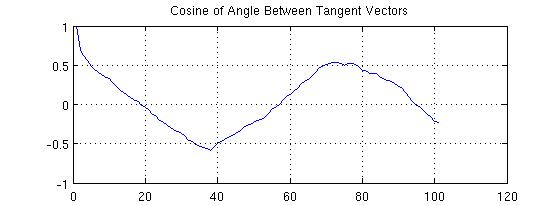
\includegraphics[width=0.9\textwidth]{chartBorder1}\\
  \caption{\ChartBord\ calculated as in \refeq{chartBordAng}. }
  \label{f:chartBorder1}
\end{figure}

\item[2012-05-11 Sebastian to Predrag]
My impression from the \statesp\ tutorial is that we first need to find
some \reqva\ to make really striking visualizations. The only
one we have right now is the trivial one, far away from the interesting
dynamics. So I think the first step is to search for them looking at
Annalisa's energy/dissipation plots. For this I think we need good charts
of the dynamics, so I will try to define more slices. Please let me know
if this is the case.

\item[2012-05-11 Predrag] I believe that at this stage exact \reqva\ are
only a distraction. You have to pick some typical snapshots of the flow
as your \templates, like you do at $\zeit=0$, to make really striking
visualizations. No need for exact solutions. This is important, because I
want experimentalist to slice their data as well, and they will never
have any exact solutions.

\item[2012-05-11 Sebastian to Ashley]
Hi Ashley!

I did used a different notation that the usual one in Chaosbook. I think
$\gSpace$ (as in \refeq{gpara}) is continuous in the physical sense, only
that it has to be regarded as discrete when one tries to implement it.
When I tried a continuous Newton-Raphson for this it failed to converge
to something meaningful. Maybe if I had followed the convention and used
something as $\gSpace' = 2 \pi \gSpace/N$ to iterate, then I would have
not had this problem.

Regarding the dot product in equation \refeq{min6} I actually got
something as in \refeq{min6_2} (I will correct \refeq{min6} afterwards).
In the code I only consider the real part of \refeq{min6_2}, however the
imaginary component is not zero. I think it should not vanish in general.
But I might be missing something, please let me know why you think it
should vanish.

I will fix the code to take advantage of the $a_m=a^*_{-m}$ property.

\item[2012-05-11 Predrag]
After you have implemented the $a_m=a^*_{-m}$ property, replot
\reffig{f:fouriervort}. Your `spectral representation' should be just the
right half, no reflection symmetry.

\item[2012-05-14 Ashley to Sebastian]
There is no need to worry about spatial discretisation,
as shifts by $\gSpace$ and inner products can all be calculated from
the data in Fourier space.

The `conjugate-symmetric' property $a_m=a^*_{-m}$ ensures that the variable $a$ is real, as
$a_m\mathrm{e}^{\mathrm{i}m\phi}
+a_{-m}\mathrm{e}^{-\mathrm{i}m\phi}$ is then a real contribution in the Fourier sum.
Now, if $a$ and $b$ are real variables, then their innerproduct must
also be real.
Most FFT libraries only return half the data for the real$\to$complex
transform ($a_m$ for $m\ge0$) and cite the conjugate-symmetric property for the rest.  I'm not sure why you have the rest of the data present.

I've scanned through the notes above, but I'm not sure what your index
$l$ is on some variables.  If you have a double-Fourier transform,
then the conjugate symmetric property is
$a_{km}=a^*_{-k,-m}$.

\item[2012-05-17 Sebastian to Predrag and Ashley]
I have been trying to implement the slice condition taking advantage of
the FFT symmetry (i.e. using only the FFT coefficients from 0 to N/2). I
manage to do so but I had to use a bunch tricks (i.e. defining a
plausible interval for the moving frame, making it always positive and
between 1 and 1024, and adding some random kick when the iteration gets
stuck in an infinite loop; all of these can be seen in the uploaded
code); they kind of make sense. I did this for a continuous version of
the Newton-Raphson algorithm; here it did not seem to be an issue. The
drifting gets removed, however the slice and {\chartBord} conditions
change dramatically, and are not as smooth any more.

The implementation was done taking only half of the values of the
transform to calculate \refeq{min4}, \refeq{min5_2}, and \refeq{min6_2}.
After all, these first $N/2+1$ coefficients are the only ones really
independent, and the rest are just complex conjugates. So maybe I just
need to consider these to build the state space vectors:
\beq
    \Re(\sspRed^\dagger \Lg \slicep)=
    \Re\left(\frac{-2 \pi i}{N} \sum_{k=0}^{N/2} \sum_{k=0}^{M-1}
    \overline{a_{lk}} a'_{lk} k e^{\frac{-2 \pi i k}{N} \gSpace}
        \right)=0
\ee{min4_2}
\beq
\Norm{\groupTan(\ssp)}^2
    = \braket{\groupTan(\ssp)}{\groupTan(\ssp)}
    = \frac{4 \pi^2}{N^2} \sum_{k=0}^{N/2} \sum_{l=0}^{M-1}
       k^2 \, \overline{a_{lk}} a_{lk}
\ee{min5_3}
and
\beq
 \braket{\groupTan(\sspRSing)}{\sliceTan{}}= \sspRed^\dagger \Lg^2 \slicep=
    \frac{4 \pi^2}{N^2} \sum_{k=0}^{N/2} \sum_{l=0}^{M-1}
    k^2 \overline{a_{lk}} a'_{lk}
\ee{min6_3}
However, I ran into serious difficulties, so I think I am doing something
wrong. In particular, the {\chartBord} condition makes no sense. It
starts at $1$ (which is expected as I start the iteration at the same
time step corresponding to the slice) and then just wonders around zero
(see \reffig{ChartBorder}).
In my previous implementation things where a lot more smoother (see
\reffig{FullFourier}), although one had to regard everything as discrete
(to see why see \reffig{SliceCondition2}). Additionally, the moving frame of both representation seems to change when looking only to a
particular time step (see \reffig{FullFourier2}), but I should look at
all the time steps to conclude about this.

I was wondering how complicated was to implement this for pipe flow, and
if you ran into similar difficulties. I will keep thinking about what is
wrong. Let me know if you have any advice.

\begin{figure}
  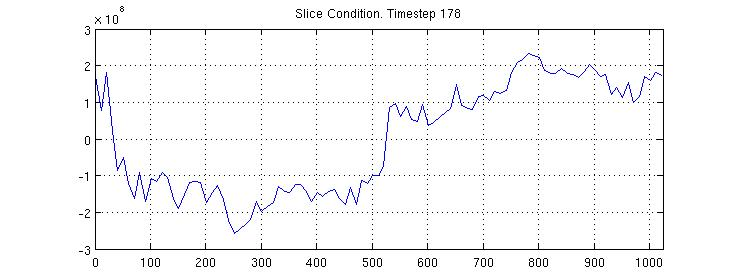
\includegraphics[width=1\textwidth]{SliceCondition}\\
  \caption{Graph of \refeq{min4} using half of the coefficients.}\label{SliceCondition}
\end{figure}

\begin{figure}
  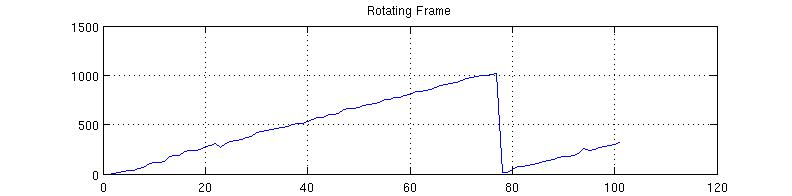
\includegraphics[width=1\textwidth]{RotatingFrame}\\
  \caption{Calculated moving frame using half of the coefficients. The jump in the moving frame is due to something I impose in the code (my moving frame is limited to change between $0$ and $1024$). I think my implementation might remove jumps of $512$ in the moving frame (equivalent to $\pi$ in the usual definition) when they occur,  as it limits the search area for the zeros of \refeq{min4_2}}\label{RotatingFrame}
\end{figure}

\begin{figure}
  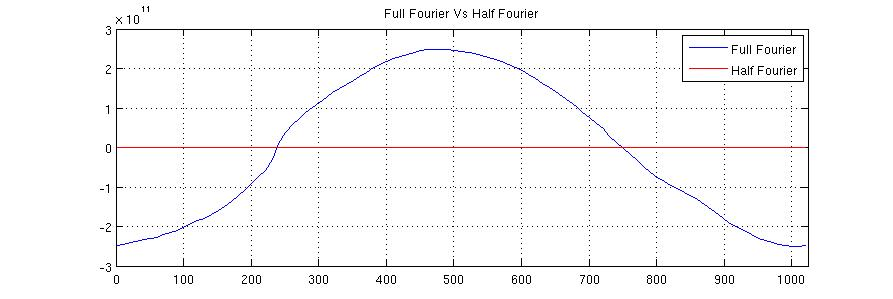
\includegraphics[width=1\textwidth]{FullFourier}\\
  \caption{Rotating frame calculated using the full coefficients of the FFT representation (Blue) and half of them (Red)}\label{FullFourier}
\end{figure}

\begin{figure}
  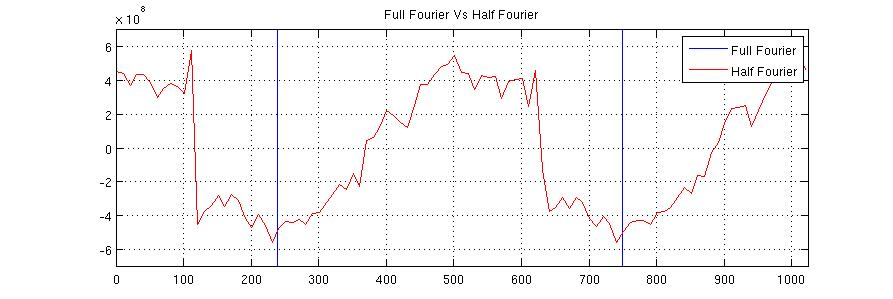
\includegraphics[width=1\textwidth]{FullFourier2}\\
  \caption{Rotating frame calculated using the full coefficients of the FFT representation (Blue) and half of them (Red)}\label{FullFourier2}
\end{figure}

\begin{figure}
  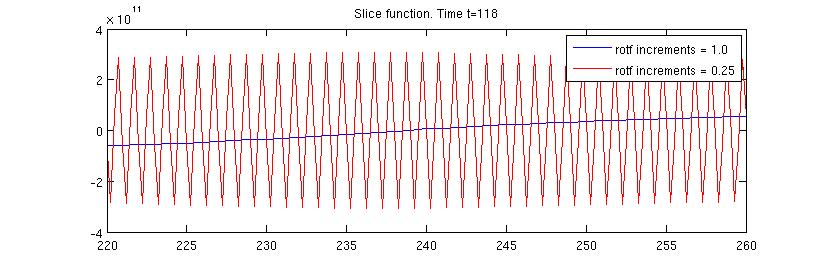
\includegraphics[width=1\textwidth]{SliceCondition2}\\
  \caption{Slice function with the full fourier representation \refeq{min4} calculated using integer values for the moving frame (Blue) and steps of 0.25 for the same variable (Red)}\label{SliceCondition2}
\end{figure}
Note: The new code is Slice2.m and sliceFunction2.m. I left the previous one for reference.

% \item[2012-05-18 Sebastian to Predrag]
% I also uploaded the code for the document I sent you. It would be great
% to talk about this. Let me know when you can.

\item[2012-06-04 Predrag]
%The doctor is in, and
\HREF{http://hint.fm/wind/}{Here} is our ultimate goal.

\item[2012-06-04 Sebastian]
%Hi Predrag! I am glad you are in again.
Great webpage. I am not sure I understand which is the ultimate goal you
are referring to; but I guess great visualizations is part of it.

\item[2012-06-04 Sebastian]
I think the discrete implementation had some issues with aliasing; I was
using frequencies higher that that of Nyquist. Nonetheless, somehow
results seemed smoother. In the DropBox uploaded movie
\texttt{BaroclinicSlice2.avi} (now in Predrag's \texttt{siminos/movies/},
not in the repository) one can see the drifting is not removed as
smoothly as before. So maybe a smaller time step needs to be considered.
But probably is because I am missing something.


\begin{figure}
\begin{center}
  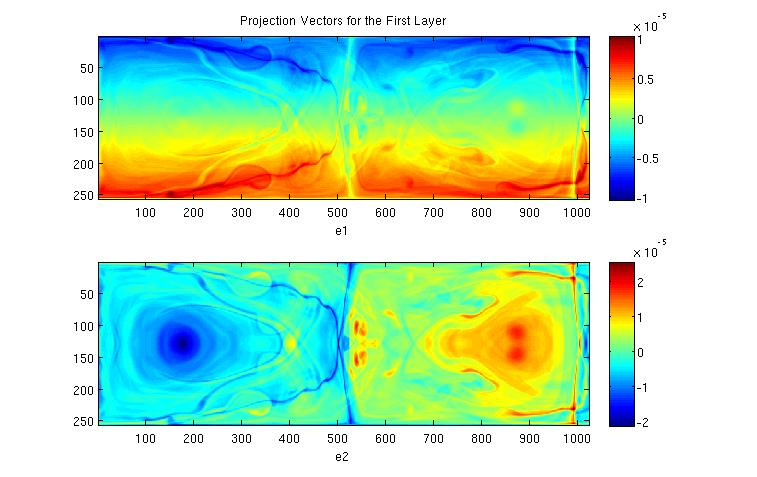
\includegraphics[width=0.9\textwidth]{Projectionvectors}
\end{center}
  \caption{orthonormal basis set
$\{\be_1, \be_2, \cdots, \be_n\}$: $\be_1$ is
  the antisymmetric vector, and $\be_2$ the symmetric one, see
  \refeq{antisymBasis}. Only the first layer is shown.
  }\label{Projectionvectors}
\end{figure}

\item[2012-06-04 Predrag]
We need to construct an orthonormal basis set
$\{\be_1, \be_2, \cdots, \be_n\}$, with $\Norm{\be_j}=1$
(using notation of \refsect{s:visualStatSp}).
We chose as a `\template' \slicep\ a `prominent state of the flow,
\[
\slicep = \bu = \bu(x,y) = \bu(x,y,\zeit) \,,
\]
an instantaneous snapshot of a steady turbulent state at arbitrary fixed
time $\zeit$.
% There is no
% streamwise reflection invariance of the flow, so I would not use $x$ reflection of
% $\bu(x,y) \to \bu(-x,y)$ in constructing
The spanwise reflection is a symmetry, so we can construct $\{\be_1,
\be_2\}$ from the orthonormal pair of vectors
\beq
\be_{1,2} = \frac{\bu(x,y) \pm \bu(x,-y)}{\Norm{\bu(x,y) \pm \bu(x,-y)}}
\,.
\ee{antisymBasis}
An example is given in \reffig{Projectionvectors}.

\item[2012-06-04 Sebastian]
I projected
trajectories onto $(\ssp_1, \ssp_2)$ using
\beq
\ssp_j = \be_{j} \cdot u =\Re \left[\sum_{n=1}^2\sum_{l=0}^{M-1}\sum_{k=0}^{N/2} u_{l,k,n} e^i_{l,k,n} \right]
\,,
\ee{dotProduct}
where $j=1,2$ defines the basis vector, $n$ accounts for the layers and
$m$ for the longitudinal direction. I uploaded the results to Dropbox's
Chaos folder. Of course, this might not mean much if the {\chartBord}
condition in \reffig{ChartBorder} is correct.

I think the movie shows some recurrences. But I am not so happy with the
slicing, and I am not sure if they really mean something, as I have to
figure out what is wrong with the implementation.

\item[2012-06-06 Predrag]
Can you read \refsect{s:chart} and use the same names?
The time steps do look too big in your current (non-orthogonalized)
$\{\ssp_1, \ssp_2\}$ projection.

% What is the `transversality
% condition' and how is it illustrated by \reffig{ChartBorder}? \ChartBord?

Do you understand {\bf [2012-05-09 Ashley]}, {\bf [2012-05-14 Ashley]} above and
agree with him? Or is your Newton still discretized? Ashley (or Gibson) will help you, if
you ask them.

The doctor is in (later today).

\item[2012-06-12 Sebastian to Predrag and Ashley]
I fixed the names in the last post. Model geometry is drawn in
\reffig{DomainDefinition}.


Newton is now continuous. However, results looked better when it was not,
and implementation was also ``cleaner'' (see {\bf [2012-05-17 Sebastian to
Predrag and Ashley]}); but this was probably for the wrong reasons.

I do understand and agree with Ashley. Nonetheless, I do still think that
taking the real part of the result in \refeq{min4} is necessary (as can
be seen in the derivation {\bf [2012-04-30 Sebastian, Predrag]}), and is
unrelated to the FFT property $a_m=a^*_{-m}$.

Recently I tried to implement the moving frame and the {\chartBord}
condition just taking into account the first $N/2$ frequencies. I did it
considering them as independent coordinates and not accounting for the
aliased frequencies given by the FFT for any sum; the results are not too
smooth. I also tried yesterday to do it taking account of this aliased
frequencies; however results do not look nice so far. Maybe, because it
is not clear to me how one should proceed. For instance given the
equation
\beq
 \braket{\groupTan(\sspRSing)}{\sliceTan{}}= \sspRed^\dagger \Lg^2 \slicep=
    \frac{4 \pi^2}{N^2} \sum_{k} \sum_{l=0}^{M-1}
    k^2 \overline{a_{lk}} a'_{lk}
\ee{min6_3_2}
one could evaluate it using $k$ form $0$ to $N-1$, or form $-N/2+1$ to
$N/2$ (or just from $0$ to $N/2$, as I did before). I think the results
will vary a lot, but maybe the second option makes more sense. I tried
yesterday to implement this; and will try again today. Is this the
correct way to do it?

% Finally, I defined an orthonormal basis as suggested above, the results
% are now in \reffig{Projectionvectors}.
I also uploaded in the DropBox uploaded movie
\texttt{BaroclinicSlice3.avi} (now in Predrag's \texttt{siminos/movies/},
not in the repository). I think reducing the
time step might be necessary.

I am not sure what is
wrong with the slicing. I believe one should be able to slice it due to
the symmetry. But maybe we need a much smaller time step, this way the
slice would be valid for more steps (if \reffig{ChartBorder} is correct,
then the slice is only valid for the first couple of time steps). Maybe
linear slices are only good for really small times in this particular
simulation.

\begin{figure}
  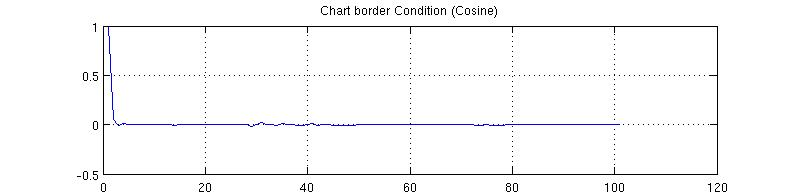
\includegraphics[width=1\textwidth]{ChartBorder}\\
  \caption{Cosine of the angle between the tangent vectors using half of
  the coefficients. This is calculated using \refeq{min5_3} and
  \refeq{min6_3}.
  }\label{ChartBorder}
\end{figure}

\item[2012-05-13  Predrag]
It might be that the chart encompassing a given \template\ is very small,
and that your \reffig{ChartBorder} is correct. Once you are gone beyond
the \ChartBord\ the orientation of the tangent vector
$\groupTan(\sspRSing(\zeit))$ in \refeq{chartBordAng} might be
essentially random compared to the $\sliceTan{}$, and in high\dmn\ vector
spaces two random vectors are nearly orthogonal. I would integrate from
$\zeit=0$ to $\zeit=4$ in very small steps, consider in more detail what
$\groupTan(\sspRSing(\zeit))$ is doing (make a movie of it).


\item[2012-06-13 Sebastian and Predrag] Following up on {\bf [2012-05-09,
2012-05-14 Ashley to Sebastian]}: Need to fix
\refeq{anti-antihermiticity}, \refeq{min4_2}-\refeq{min6_3},
\refeq{dotProduct}, \refeq{min6_3_2}, evaluate using $k$ from $-N$ to $N$
(instead of $0$ to $N$), then use $a_m=a^*_{-m}$ and/or
$a_{km}=a^*_{-k,-m}$ to prove that all dot product of vectors that you
compute are real numbers (due to the reality of $u(x,y)$, with no need to
impose \refeq{120430_11}). In particular, \refeq{anti-antihermiticity} is
wrong, fix it.

\item[2012-05-13  Predrag]
From \texttt{BaroclinicSlice3.avi}, and the simultaneous projection on the
$\{\ssp_1, \ssp_2\}$ (in basis of \reffig{Projectionvectors}), it is clear
that the time steps are gigantic - need to integrate in fine steps for
one large structure turnover time,
$\Delta\zeit = 10-100$.

The situation is much more difficult than in the (very smooth) pipe flows
near onset of turbulence. The picture that is emerging is a large,
lumbering wall to wall structure, with very fast small vortices on top of
it. Hopefully they act as noise, and smear the the \statesp\ trajectory
of the large structures. Perhaps it is these vortices that make a chart
in \reffig{ChartBorder} so short-lived; so new thinking is needed.

Our first goal would be to find a smooth (no fine vortices) \reqv\
solution, use it to replace \reffig{Projectionvectors}.

\item[2012-07-16 Sebastian]
I went over the implementation, and I think I had a problem with the
theory but end up doing the right thing in practice. DFT is
defined as:
\beq
\widetilde{f}_k=\frac{1}{N}\sum_{j=0}^{N-1} f(x_j) e^{-2 \pi i j k/N}
\ee{DFT1}
for $k=-N/2,....,N/2-1$. And the synthesis equation as:
\beq
f(x_j)=\sum_{k=-N/2}^{N/2-1} \widetilde{f}_k e^{2 \pi i j k/N}
\ee{DFT2}
for $j=0,1,2,\cdots,N-1$. Then the vorticity is expanded as:
    \beq
    \xi(x_j,y)=\sum_{k=-N/2}^{N/2-1} a(y)_{k} e^{-2 \pi i k j/N}
    \ee{fft1}
and we have to consider the coefficients $a(y)_k$ for frequencies from
$k=-N/2,\cdots,N/2-1$. This leads to the slice condition:
    \PC{$[-N/2,\cdots,N/2-1]$ is a strange range? Sebastian: It is the
    definition some authors give to the DFT (see for instance Chapter 1
    of Kopriva\rf{SpectralPDE}; one can get it electronically trough
    Gatech library webpage) probably it is done this way in order to
    avoid multiplying the coefficients related with $N/2$ and $-N/2$ by
    $1/2$. Other authors use the range $[0,\cdots,N-1]$.}
\beq
    \sspRed^\dagger \Lg \slicep=
    -\,\frac{2 \pi i}{N} \sum_{k=-N/2}^{N/2-1} \sum_{l=0}^{M-1}
    \overline{a}_{lk} a'_{lk} \, k \, e^{-\,\frac{2 \pi i k}{N} \gSpace}
     =0
\,,
\ee{rot_frame}
but since we have the property $a_{l,m}=a^*_{l,-m}$ the imaginary numbers
cancel by pairs, so that we might as well compute:
\beq
    \sspRed^\dagger \Lg \slicep=
    2 \cdot \Re\left(\frac{-2 \pi i}{N} \sum_{k=0}^{N/2} \sum_{l=0}^{M-1}
    \overline{a}_{lk} a'_{lk} \, k \, e^{-\,\frac{2 \pi i k}{N} \gSpace}\right)
     =0
\,,
\ee{rot_frame2}
where taking the real part is just a trick to reduce computations. This
is what it is implemented  in \verb"Slice2.m" and
\verb"SliceCondition2.m". Only the factor of $2$ is missing, but that
would not change the results at least qualitatively. This would imply
that \refeq{min4_2}--\refeq{min6_3}, \refeq{dotProduct}, \refeq{min6_3_2}
are correct (except for the factor of $2$). But I might be missing
something.

\item[2012-07-17 Predrag]
Seems OK (have not checked the algebra). Weird - I did not get email
about your edit. Are you getting them? (we just changed the server, there
could be configuration problems).

\item[2012-07-17 Predrag]
What is `synthesis equation'? Sebastian: It is another way to refer to the inverse of the DFT.
Predrag:
\HREF{http://www.dspguide.com/ch8/5.htm}{Google agrees}.


\item[2012-07-16 Sebastian]
I will talk to Annalisa to download the code from her computer and run it
in mine, or in the server, with smaller time steps. Not sure how to look
for the relative equilibrium, but I guess smaller time steps are needed
first.

\item[2012-07-17 Predrag]
Talk to her ASAP, as she is leaving for Italy soon (for 2-3 weeks?).
We have a linux server, if you need access (also to PACE cluster).

\item[2012-07-17 Sebastian]
Hi Predrag. I did get the email. {\bf [2012-07-17 Predrag]} Weird - I did
not get alert of your last edit either (but get all others...).

I talked to Annalisa and have the code; she pointed out we might only
need to decrease the saving intervals of the simulation and not the
time-step per se.

I am now struggling to get the FFTW libraries to work on my computer. It
might be easier on the server if the libraries are already installed on
it.

\item[2012-07-19 Sebastian]
I ran the code saving the output $10$ times more frequent than before. As
expected, the slicing is much more smooth now, and the {\chartBord}
condition is valid for more time-steps. However the slices remain only
valid for short times (see \reffig{ChartBorder2}\,(a)).

\item[2012-07-19 Predrag] Great simulation! Not having the movie but steps
is quite helpful in looking at. Can you try this: instead of plotting
the flow in the slice, plot the bit-by-bit differences between the two videos:
it will start out white, but as you go away from the template state, it will
show you only the regions where there is the fastest change; we need to understand why
the small structures can drive you to the \chartBord.

Please check out repository \texttt{pipes} (you are sortega = baroclinic
there as well), and read pipes/blog/blog.pdf starting with {\bf
[2012-05-30 Humbledt]}. You will see the same behavior for the pipe flow,
but I do not believe there are small structures in that problem.



\item[2012-07-19 Sebastian]
I also modified the code to redefine the slice when necessary, only to
see how long are different slices valid (as have been done for pipe
flow). I am uploading \texttt{multipleSlices.pdf} to dropbox (did not
figure out how to make a movie here). I think what is seen is that
drifting combined with the thin filaments and small vortices is the main
reason for which the slices are not valid for long. I was wondering if
there is possible to overcome this issue by defining something as a
moving slice (along group orbits), but I am not sure how the charting
would work in this case. I will keep thinking about this.

\item[2012-07-19 Predrag] As you will see in the pipes/blog/blog.pdf, I've
been thinking the same way (looks like there is a rotating structure, so
perhaps there is a rotating frame with charts valid for much longer times),
but I think you have a better idea - we need to understand what is it that
makes $\cos \theta$ go to zero so fast.

\item[2012-07-19 Predrag]  Weird - when you commit, I do not get email
about your edit. Do you? Forward it to me if you do. Yours is the only
email that svn refuses to forward to me...

\item[2012-07-25 Predrag]
So far we are measuring the distance $|\ssp|^2=\braket{\ssp}{\ssp}$ in
terms of the Euclidean inner product
\beq
\braket{\ssp}{\slicep} = \sum_i^d {\ssp}_i \slicep_i
    \,,\; \qquad
x, y \in \pS \subset \reals^d
	\,.
\ee{innerR}
Any representation of a compact group $\Group$ is fully
reducible\rf{Hall03}. The invariant tensors constructed by contractions
of $\Lg_a$ are useful in identifying irreducible representations. The
simplest such invariant is
\beq
{\Lg}^{\dagger} \cdot \Lg = \sum_m C_2^{(m)} \, \id^{(m)}
\,,
\ee{QuadCasimir}
where $C_2^{(m)}$ is the quadratic Casimir for irreducible representation
labeled $m$, and $\id^{(m)}$ is the identity on the irreducible subspace
$m$, 0 elsewhere. For compact groups $C_2^{(m)}$ are strictly
nonnegative. $C_2^{(m)} =0$ if $m$ is an invariant subspace. For \SOn{2}
it is simply $C_2^{(k)} =k^2$, $\id^{(m)}$ is $[2\!\times\! 2]$ unit matrix,
where $k$ refers to the $k$th Fourier
mode.

The dot product of two tangent fields in \refeq{min4} is a sum of inner
products weighted by Casimirs \refeq{QuadCasimir}, as in \refeq{min5}
\beq
\braket{\groupTan(\ssp)}{\groupTan(\slicep)}
   = \sum_m C_2^{(m)} {\ssp}_i\, \delta_{ij}^{(m)} \slicep_j
\,.
\ee{braket0}
The slice condition thus preferentially weighs higher Fourier modes. If
we think of the norm as the Sobolev $H^{-1}$ norm, it would be natural to
have it as unit norm on the product of tangents, which  means we should
change \refeq{innerR} to
\beq
\braket{\ssp}{\slicep}
   = \sum_m {\ssp}_i\, \frac{\delta_{ij}^{(m)}}{C_2^{(m)} } \slicep_j
\,.
\ee{braket}
This would suppress higher Fourier modes, on hopefully tame the fast
rotations observed by Ashley and Sebastian in pipe, respectively
baroclinic  flows.

{\color{red} Please try it!} a very simple change in the slicing condition that
should reduce the number of charts along short recurrent orbits.

\item[2012-07-26 Sebastian] I uploaded to the DropBox.com a movie showing
the difference between the simulation on full state space and on the
slices. It shows that the larger differences are in the two thin
filaments that cross the domain.

\begin{quote}
\HREF{../movies/BaroclinicSlice4.avi}{../movies/BaroclinicSlice4.avi}.
\end{quote}

\item[2012-07-27 Predrag] The movie is very helpful. It shows clearly
that it is the fine structure that causes charts to be small. As the
Sobolev $H^{-1}$ norm carries all of the spectral information, I think it
is legal.

\item[2012-07-26 Sebastian] I think I understand the essence of what you
want to say in \textbf{[2012-07-25 Predrag]} (and would like to know more
about the theory; I will look in the cited reference). It appears to me
that what you are proposing, in practical terms, is similar to filtering
the series so that the gravest modes contribute more in the dot product.

I will work out the math for equations \refeq{min4} and \refeq{min5} and
post it online. As a first guess I think I would get something as:
\beq
    \sspRed^\dagger \Lg \slicep=
    2 \cdot \Re\left(\frac{-2 \pi i}{N} \sum_{k=0}^{N/2} \sum_{l=0}^{M-1}
    \frac{\overline{a}_{lk} a'_{lk} \, e^{-\,\frac{2 \pi i k}{N} \gSpace}}{k}\right)
     =0
    \,,
\ee{min4_4}
    for \refeq{min4} and
\beq
    \Norm{\groupTan(\ssp)}^2
    = \braket{\groupTan(\ssp)}{\groupTan(\ssp)}
    = \frac{4 \pi^2}{N^2} \sum_{k=0}^{N/2} \sum_{l=0}^{M-1}
       \, \overline{a_{lk}} a_{lk}
\ee{min5_3}
\beq
    \braket{\groupTan(\sspRSing)}{\sliceTan{}}= \sspRed^\dagger \Lg^2 \slicep=
    \frac{4 \pi^2}{N^2} \sum_{k=0}^{N/2} \sum_{l=0}^{M-1}
    \overline{a_{lk}} a'_{lk}
    \ee{min6_3}
for the other equations. It seems to be a very good solution, I will
implement it. I was wondering about the drawbacks, if any, of the Sobolev
$H^{-1}$ norm.

\item[2012-07-27 Predrag] The powers of $k$ look correct.

\item[2012-07-26 Sebastian, as a Side Note]  I was reading today about
how the Madden Julian Oscillation (MJO) is forecasted, and its phases
tracked; and I think they do something similar, to what you are
proposing, using Empirical Orthogonal Functions (EOF). I believe the
process is something as making composites of time-filtered series of data
(20 to 60 day filter), obtaining the EOF's, and then comparing real time
data to these functions to get the phase of the MJO (for this they
project to a 2 dimensional space). I will learn more about this in the
Fall (I am taking data analysis then). I think it would be interested to
see how all this relates to the dynamics.

\item[2012-07-27 Predrag] My impression is that `filtering' refers to
deleting parts of the Fourier spectrum. Here we keep all of it, but with
a weight gives less importance to high-frequency components.

\item[2012-07-27 Predrag]                       \toCB
Hopefully the \chartBord\ for the the Sobolev $H^{-1}$ norm lies further out from the
template than the one for the Euclidean norm: the idea is the amplitude
of the higher mode in the 'baseball seam' of Fig.~7\,(a) in
\HREF{http://www.cns.gatech.edu/~predrag/papers/atlas12.pdf}
{\refref{atlas12}} is suppressed, so the \template\ neighborhood goes
further out before it hits the first group-orbit wiggle.

It seems to work for Ashley - here are two posts from
\texttt{pipes/blog/}:

\item[2012-05-22 Ashley]
 %Started experimenting with $\slicep{}^{(1)} = a(0)$.
% % , then   tried adding $\slicep{}^{(2)}=\sspRed(6)$;
% % cf.\ \reffig{fig:A29-2tmplts}.
% The problem is that $\cos\psi$ might
% suggest that $\slicep{}^{(2)}$ is within the boarder of
% $\slicep{}^{(1)}=\sspRed(0)$, but I don't know how to tell in
% advance that $\slicep{}^{(1)}$ will be within the
% boarder of $\slicep{}^{(2)}$.  It switched but then has
% jumps before reaching $t=6$.
% I also wan't sure that I was tracking the
% appropriate root for the second template before the switch.
% Searching though the possible roots of the slice
% condition for the templates, other than the current template,
% fixes that, but is a lot of work.
 I've played with adding templates on the fly in
 \reffig{fig:3610switching}\,(a).  At the end of the orbit
 it didn't switch back to the first template --- I've only permitted
 switching when shifts match for a closer template.  The shifts
 often run side by side but don't cross.

\item[2012-07-27 Ashley]
The Sobolev $H^{-1}$ norm avoids need for a bunch of templates
to navigate around $\RPO{36.72}$.  See \reffig{fig:3610switching}\,(b),
in particular the red line.  Compare with \reffig{fig:3610switching}\,(a).


\item[2012-07-27 Sebastian]
I did the slicing with the proposed weights. The equations I end up using are:

\beq
    \sspRed^\dagger \Lg \slicep=
    2 \cdot \Re\left(\left(\frac{-2 \pi i}{N}\right)^{-1} \sum_{k=1}^{N/2} \sum_{l=0}^{M-1}
    \frac{\overline{a}_{lk} a'_{lk} \, e^{-\,\frac{2 \pi i k}{N} \gSpace}}{k}\right)
     =0
    \,,
\ee{min4_5}
    for \refeq{min4} and
\beq
    \Norm{\groupTan(\ssp)}^2
    = \braket{\groupTan(\ssp)}{\groupTan(\ssp)}
    = \sum_{k=1}^{N/2} \sum_{l=0}^{M-1}
       \, \overline{a_{lk}} a_{lk}
\ee{min5_5}
\beq
    \braket{\groupTan(\sspRSing)}{\sliceTan{}}= \sspRed^\dagger \Lg^2 \slicep= \sum_{k=1}^{N/2} \sum_{l=0}^{M-1}
    \overline{a_{lk}} a'_{lk}
    \ee{min6_5}
Note that I changed the sum related to $k$ so that it goes from $1$ to
$N/2$. It worked (see \reffig{ChartBorder3}\,(b)) and now the slice is valid
for much longer times, but I am not sure if we can just ignore the
singularity for $k=0$ in the slice condition. However, with the previous
norm this mode was always canceled out; so it might be OK.

\item[2012-07-26 Predrag] Looks much better! In anything that has a
factor of \Lg\ $m=0$ is removed. However, our derivation of slice starts
with minimizing the distance $\norm{\ssp-\slicep}^2$, so please set the
$m=0$ part of the norm to $1$ until we show that is right or think of an
alternative.

 \begin{figure}
 \begin{center}
(a) 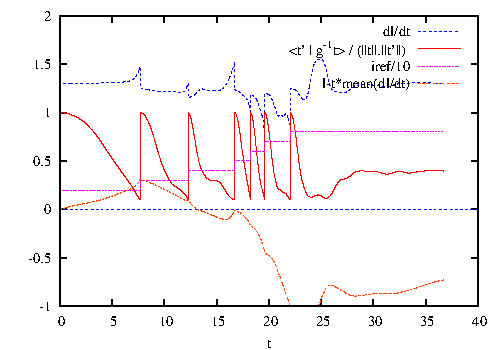
\includegraphics[width=0.90\textwidth]{3610switching}
 \\
(b) 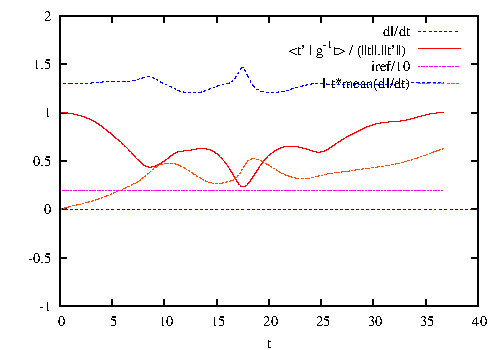
\includegraphics[width=0.90\textwidth]{3611switching}
 \end{center}
 \caption{ \label{fig:3610switching}
 {\ChartBord} condition for the pipe flow \rpo\ $\RPO{36.72}$
 discovered in \refref{ACHKW11}:
    (a) [2012-05-22 Ashley]
    Tracking $\RPO{36.72}$ starting with $\slicep{}=\ssp(\zeit=0)$ and
    adding new templates on the fly, whenever $\cos\psi<0.1$.
    (b) [2012-07-27 Ashley]
        Tracking $\RPO{36.72}$ starting with $\slicep{}=\ssp(\zeit=0)$. Just as
    in frame (a), except here using the Sobolev $H^{-1}$
    norm;
    %\refeq{eq:dampednorm};
    $\cos\psi$ does not drop below $0.1$.
 }
 \end{figure}

\begin{figure}
(a) 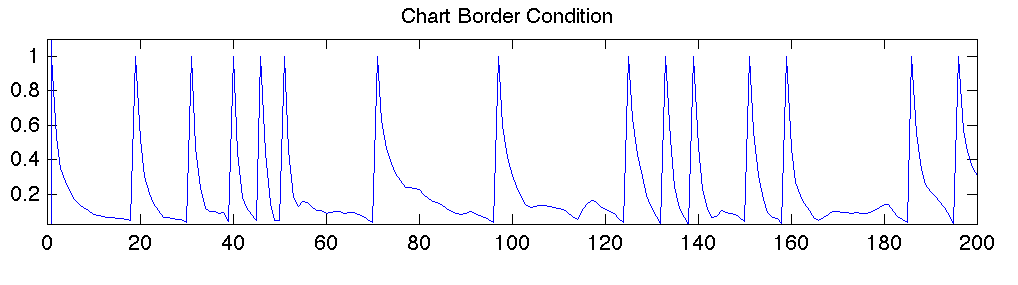
\includegraphics[width=0.92\textwidth]{ChartBorder2}
    \\
(b) 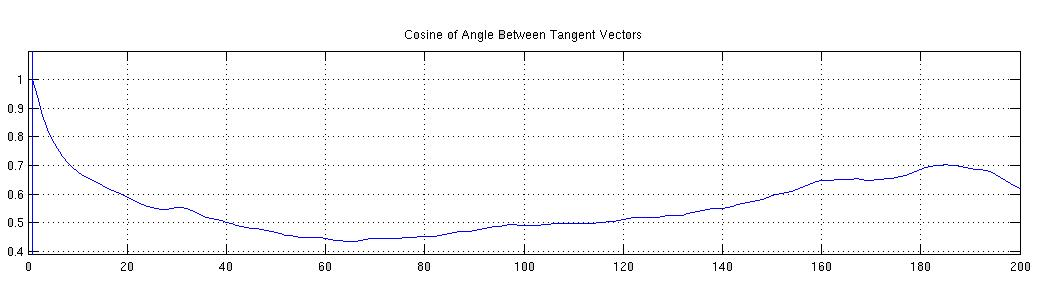
\includegraphics[width=0.9\textwidth]{ChartBorder3}
    \\
(c) 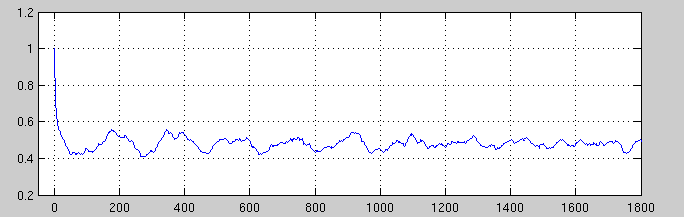
\includegraphics[width=0.9\textwidth]{ChartBorder4}
  \caption{{\ChartBord} condition for the baroclinic
  instability\rf{BrCv12}. The current state is used as the new \template\
  each time the $\cos$ of the angle between the two tangent vectors
  \refeq{chartBordAng} is smaller than $0.05$.
(a) [2012-07-19 Sebastian] Using the energy norm.
(b) [2012-07-27 Sebastian] Using the Sobolev $H^{-1}$ norm  \refeq{braket}.
(c) [2012-08-21 Sebastian] A long run with the Sobolev $H^{-1}$ norm.
}\label{ChartBorder2}
\end{figure}


\item[2012-07-26 Predrag] I think we can probably make a good argument
that the group manifold should be a
\HREF{http://en.wikipedia.org/wiki/Sobolev_space\#Sobolev_spaces_with_integer_k}
{Sobolev space} $W^{1,\infty}$ with respect to group parameter
derivatives - the group orbit is a smooth manifold. I have argued some
time ago for Ruslan Davidchack somewhat inchoately that for \KS\ Fourier
expansion of $u(x)$ ({\bf [2012-03-25 Predrag to Evangelos]}) that the
important, nonlinearly coupled ``Fourier modes contribute significantly
for any magnitude not smaller than $1/m$ for the $m$th mode''. If they do
this for $k \to \infty$, the partial derivative $u_x$ is not defined, and
that would be a disaster. Which probably means for Navier-Stokes that we
can demand that solutions belong to $W^{2,\infty}$ which would make it
legit to use even stronger suppression of high Fourier modes, with the
Sobolev $H^{-1}$ norm diagonal $\propto (C_2^{(m)})^{-2}$.

\item[2012-07-27 Sebastian]
The new norm seems to solve the problem. However I have doubts about what
should we do with $k=0$.

\item[2012-07-27 Predrag]
For now, keep $k=0$ term in the norm $=1$. It think we need it.

\item[2012-08-03 Predrag]
\HREF{http://www.math.wisc.edu/~jeanluc/preprints.html} {Jean-Luc
Thiffeault} reviews Sobolev norms in Sect.~3 of \arXiv{1105.1101}.

Can you do the movie of the sliced flow in the negative Sobolev norm,
together with the norm of the difference between sliced and full
\statesp? This time there should be no wild jumps as one seem to never
get close to the chart border...

\item[2012-08-21 Sebastian]
I did the slicing with the the Sobolev $H^{-1}$ norm  \refeq{braket} for
a much longer simulation. The slice seems to be valid for a really long
time (see \reffig{ChartBorder3}\,(b)). This is kind of weird I believe;
but I have not give it a good though. I have to review the norm paper for
this, as probably it is an issue with the implemented norm.

\item[2012-08-21 Predrag]
OK, you win - I cannot download your attachments (Beijing does things to
gmail) and enter them into blog, so for this once you get email rather
than a blog entry:

If we are not paying some other price for this, this might be the best
news every: a single slice suffices! However, the differences between
\reffig{ChartBorder3}\,(b) and (c) worries me: graph (b) dips much lower,
and (c) is suspiciously above 0.4 for all times...

Remember, when  you go back to spatial representation to reconstruct the
video for reduced dynamics, you have to use the inverse of the norm (I
believe). Curious what that looks like now....

\item[2012-07-30 Sebastian]
I was wondering if you would like to form part of my thesis advisory
committee. I am thinking in looking for periodic orbits in models of the
MJO as described in \emph{PeriodicOrbitsClimate.tex}\PC{missing *.bib
entries for "Lorenz60" and "Webster72"} I added to the repository some
days ago. As a starter I am thinking in looking at a simple
Stechman\rf{StMaKh08}  2008 model (you can search for it on
Majda's \HREF{http://math.nyu.edu/faculty/majda/publicationrevised.html}
{homepage}). I am working towards implementing an spectral version of the
equations.

\item[2012-07-30 Predrag] These guys have written zillion related papers
since, make sure you read the relevant ones first. I have officemates in
GFD Woods Hole program I'll ask about these papers.

\item[2012-08-03 Predrag] That would be great, will gladly join. Remember to
apply for GFD Woods Hole Fellowship coming Fall / Spring, that would be
a good place for you next summer.

\item[2012-08-06 Sebastian]
I have been trying today to do the slicing for the whole simulation,
however I have been ruining into some trouble with the size of the files.
But I will get it done. I might also run another simulation to get more
time steps.

Regarding the applications to the MJO. I found a very simple model one
might start exploring (Majda and Stechmann\rf{MajSte11}, \emph{Nonlinear
dynamics and regional variations in the {MJO} skeleton}). I think is
better to explore this one than the one I coded up for gravity waves. As
the former has nonlinearities related to advection terms; the later is
simpler to analyze.

\item[2012-08-07 Sebastian]
Thanks for joining! I am very happy with the committee, it would be conformed
by Peter, Annalisa and yourself. Surely a great one.

I will apply to Woods Hole next summer. It seems to be a great experience.
And the topics are very interesting.

The paper looks really nice. I had been a bit lost trying to find a place
to study these topics. But this one seems to solve the issue. I will let
you know how it goes.

\item[2012-08-21 Sebastian]
Please find the \HREF{PeriodicOrbitsClimate/ExplRecStructs.pdf}
{presentation} I gave to the group of what I want to do for the Phd.
There I show results of the two models I told you about (the gravity wave
and the MJO models). Due to size constraint I removed the videos. However
I uploaded one to Dropbox and the other one you have it already. Let me
know what you think. Note that models would need additional tweaking
before being use, in order for them to be representative of the physics.
And that maybe another model might be better. I wrote Professor Majda at
NYU asking which he considered the best one. No answer yet, so I might
write again.

I am not sure how my work dynamics will be this semester. I will be
taking 2 classes, working as a TA and working on the proposal. But I am
sure it will workout somehow. It will be nice to get together and set
some goals.

\item[2012-07-27 Sebastian]
\item[2012-08-03 Predrag]



\end{description}
